\documentclass[11pt]{article}
\usepackage[margin=1in]{geometry}
\usepackage{fontspec}
\setmonofont[Path=fonts/]{DejaVuSansMono.ttf}
\usepackage{amsmath,amssymb,amsthm,mathtools}
\usepackage{graphicx,booktabs,hyperref}
\usepackage{fvextra}
\hypersetup{hidelinks}
\newtheorem{theorem}{Theorem}
\newtheorem{lemma}{Lemma}
\newcommand{\C}{\mathbb{C}}
\newcommand{\ket}[1]{\lvert #1\rangle}
\title{Power and Cosine Filtering for Extreme Singular-Value Estimation:\\
An Assumption-Aware Technical Reassessment of a QSVT Proposal}
\author{[Author name and affiliation to be supplied]}
\date{Internal technical-report draft\\26 October 2026}
\begin{document}
\maketitle
\begin{abstract}
We reassess an unpublished proposal for quantum maximum/minimum singular-value estimation, focusing on its cosine-based triangular iteration. For a rectangular matrix $A$, we formulate the method on the normalized right Gram operator $G=(A/\alpha)^\dagger(A/\alpha)$, where $\alpha\geq\|A\|$ is an available normalization bound. A bounded even polynomial approximation to $\cos(\beta G)$ is a candidate target for a polynomial eigenvalue transformation, subject to an explicit QSP completion and normalization convention. We prove a finite-spectrum filtering bound: if the input has weight $a>0$ on the minimum-eigenvalue eigenspace and the largest non-target filter response is at most $r<1$ times the target response, then the conditional leakage is at most $(1-a)r^{2t}/a$ after $t$ iterations. A Bernoulli block-encoding readout estimates the filtered Gram expectation and converts its additive error into a singular-value error bound. The result depends on target overlap, spectral separation, postselection success, normalization, and readout precision; it is not a circuit-level or end-to-end complexity theorem. Small matrix-level simulations reproduce the predicted convergence and its failures for zero overlap, narrow gaps, and right kernels. We also compare the original $\cos(\beta(\sigma/\alpha)^2)$ response with a distinct dilation-based $\cos(\beta\sigma/\alpha)$ variant. No QSVT phases or quantum circuits are synthesized, and no quantum speedup or novelty claim is made.
\end{abstract}
\section{Introduction}
Extreme singular values arise in numerical linear algebra and in spectral questions connected to ground-state energy estimation. An earlier manuscript, \emph{Quantum maximum/minimum singular-value estimation algorithms} (author and publication metadata not stated in the source file; hereafter QMSVE) proposes quantum power iteration for the largest singular value, an inverse-iteration baseline for the smallest, and a cosine-based triangular iteration that avoids explicitly applying a matrix inverse \cite{QMSVE}. This report makes that proposal precise on a right-space operator, records the conditions needed for convergence, and checks a small set of finite-dimensional examples.

The main correction is about the operator being transformed. For a general rectangular matrix, applying $\cos(A)$ is not a valid singular-value prescription. We instead set $B=A/\alpha$ and $G=B^\dagger B$ on the right singular-vector space. The QMSVE cosine rule is then $C=\cos(\beta G)$, whose eigenvalues are $\cos(\beta\sigma_i^2/\alpha^2)$. This function is positive and decreasing on the normalized spectrum when $0<\beta<\pi/2$. A Hermitian-dilation construction gives a different response, $\cos(\beta\sigma_i/\alpha)$; we keep it separate.

Our contribution is a careful statement and finite-spectrum proof of conditional filter convergence, its measurement-to-energy conversion, and a reproducible matrix-level audit. It does not establish that the original proposal is new, that its full resource estimate is correct, or that it outperforms existing algorithms. In particular, a gap and nonzero initial overlap remain essential, while each successful filtered sample may require many fresh attempts.
\section{Related work and scope}
Quantum singular-value transformation (QSVT) implements bounded polynomial transformations of singular values of a block-encoded matrix, and the Hermitian specialization implements polynomial eigenvalue transformations \cite{Gilyen}. It supplies a possible implementation primitive for the polynomial cosine filters considered here; the present work does not synthesize its phase angles. Quantum power methods and quantum inverse iteration already have substantial prior literature \cite{SekiYunoki,Kyriienko,Nghiem}. These works differ in input and implementation models, but they rule out treating power iteration or QSVT-based powers as new in themselves.

The QMSVE manuscript is an unpublished source document with no author or venue metadata in the copy examined. Its triangular iteration is marked provisional. We therefore treat it as the origin of the algorithmic idea being reassessed, not as a verified theorem or a published result. The author's separate QCG work is cited only as prior project context and is not conflated with this method \cite{QCG2023,QCG2024}.
\section{Model and algorithm}
Let $A\in\C^{m\times n}$, $m\geq n$, and choose a known $\alpha\geq\|A\|_2>0$. Define
\[
 B=A/\alpha,\qquad G=B^\dagger B,\qquad
 0\leq \lambda_0\leq\lambda_1\leq\cdots\leq\lambda_{n-1}\leq1,
\]
where $\lambda_i=\sigma_i(A)^2/\alpha^2$ are the eigenvalues of $G$ in increasing order. The target is the smallest singular value over the full right space, including zero modes. Estimating the smallest nonzero singular value requires an additional promise or access to the kernel-orthogonal subspace. For wide matrices ($m<n$), the right Gram operator necessarily has a kernel, so the same distinction applies.

Let $\ket{\psi}=\sum_i c_i\ket{v_i}$ be a normalized input state in a right singular basis and set $p_i=|c_i|^2$. For $0<\beta<\pi/2$, the ideal cosine-Gram filter is
\[
 C=\cos(\beta G),\qquad q_i=\cos(\beta\lambda_i)\in(0,1].
\]
The unnormalized state after $t$ iterations is $C^t\ket{\psi}$, its ideal success probability is
\[
 Z_t=\|C^t\ket{\psi}\|^2=\sum_i p_i q_i^{2t},
\]
and the normalized accepted state's spectral weights are $p_iq_i^{2t}/Z_t$. This is the QMSVE rule applied to the right Gram operator, with normalization made explicit.

\paragraph{Polynomial implementation model.}
For an integer $m_0\geq0$, let
\[
 P_{m_0}(x)=\sum_{j=0}^{m_0}\frac{(-1)^j(\beta x)^{2j}}{(2j)!},
 \qquad
 \delta_{m_0}=\frac{\beta^{2m_0+2}}{(2m_0+2)!},\qquad
 \widetilde P_{m_0}(x)=\frac{P_{m_0}(x)}{1+\delta_{m_0}}.
\]
The polynomial $P_{m_0}$ is the Maclaurin polynomial of $\cos(\beta x)$ through degree $2m_0+1$ (the odd coefficient vanishes). Taylor's theorem and the bound on every derivative of cosine give $|P_{m_0}(x)-\cos(\beta x)|\leq\delta_{m_0}$ for $|x|\leq1$. Hence $|\widetilde P_{m_0}(x)|\leq1$ on $[-1,1]$ and $\|\widetilde P_{m_0}-\cos(\beta\,\cdot)\|_\infty\leq2\delta_{m_0}/(1+\delta_{m_0})$; $\widetilde P_{m_0}$ is even of degree $2m_0$. It is therefore within the standard bounded-polynomial Hermitian-QSVT class for a block-encoding of $G$ \cite{Gilyen}. This establishes an admissible polynomial response, not a phase sequence, gate synthesis, or a compiled circuit. As a polynomial in the singular value $\sigma/\alpha$, the response $\widetilde P_{m_0}((\sigma/\alpha)^2)$ has degree $4m_0$.

If a block-encoding of $B$ is available, a product construction can encode $G=B^\dagger B$ using two calls to the $B$ encoding, up to ancilla and reflection costs. We write $d_G$ for the actual oracle-query cost of one implemented cosine-polynomial transform of $G$, and $c_\psi$ for state preparation. Neither is numerically estimated here. A coherent implementation of $t$ transforms has query depth proportional to $t d_G$; a hard depth cap therefore constrains $t$ as well as the polynomial degree. The normalization bound $\alpha$ and its acquisition cost are inputs, not free outputs of this method.

\section{Finite-spectrum convergence and readout}
Let $T=\{i:\lambda_i=\lambda_0\}$ be the minimum-eigenvalue eigenspace, with initial mass $a=\sum_{i\in T}p_i>0$. Let $q_*=\cos(\beta\lambda_0)$ and suppose
\[
 q_i\leq r q_*\quad(i\notin T),\qquad 0\leq r<1.
\]
For the cosine-Gram response, if an eigenvalue strictly larger than $\lambda_0$ exists, define $\lambda_+=\min\{\lambda_i:\lambda_i>\lambda_0\}$; then $r=\cos(\beta\lambda_+)/\cos(\beta\lambda_0)<1$. If no such eigenvalue exists, all spectral weight is already in the target subspace and $F_t=1$.

\begin{theorem}[Conditional spectral leakage]
For every integer $t\geq0$, let $F_t$ be the probability mass of $T$ in the normalized state $C^t\ket{\psi}/\sqrt{Z_t}$. Then
\[
 1-F_t\leq\frac{1-a}{a}r^{2t}.
\]
If $\mu_t=\langle C^t\psi|G|C^t\psi\rangle/Z_t$, then
\[
 0\leq\mu_t-\lambda_0
 \leq(1-\lambda_0)(1-F_t)
 \leq\frac{1-a}{a}r^{2t}.
\]
\end{theorem}

\noindent The proof is given in Appendix~\ref{app:proof}. Lean formalization is in progress; Appendix~\ref{app:lean} will state its exact scope and checker status. The identification of the finite weights with a matrix eigenbasis, the block-encoding implementation, and the readout interpretation are finite-dimensional mathematical derivations, not part of the scalar Lean theorem.

\paragraph{Finite-degree transfer condition.}
The leakage theorem also applies to a bounded polynomial response $\widetilde q_i=\widetilde P(\lambda_i)$, but boundedness alone does not ensure that it orders the target eigenvalue correctly. Let $q_{\mathrm{out}}=\max_{i\notin T}q_i$ and let $E$ be a uniform error bound $|\widetilde P(x)-\cos(\beta x)|\leq E$ on $[0,1]$. If $E<(q_*-q_{\mathrm{out}})/2$, then $|\widetilde q_*|\geq q_*-E>0$ and $|\widetilde q_i|/|\widetilde q_*|\leq(q_{\mathrm{out}}+E)/(q_*-E)<1$. The generic finite-weight bound therefore transfers with this ratio. This sufficient condition can be conservative and is not evaluated as a degree-optimal filter here.

\paragraph{Maximum-singular-value branch.}
For the power method, take response $q_i=\lambda_i$ and target the maximum eigenspace $T_{\max}=\{i:\lambda_i=\lambda_{\max}\}$. If its initial mass is $a_{\max}>0$, $\lambda_{\max}>0$, and $\lambda_-=\max\{\lambda_i:\lambda_i<\lambda_{\max}\}$ exists, the same finite-weight inequality applies with $q_*=\lambda_{\max}$ and $r=\lambda_-/\lambda_{\max}$. Its target leakage is at most $((1-a_{\max})/a_{\max})r^{2t}$, and its filtered mean obeys $0\leq\lambda_{\max}-\mu_t\leq(1-F_t)\leq((1-a_{\max})/a_{\max})r^{2t}$. The maximum singular value estimate is $\alpha\sqrt{\widehat\mu_t}$ with corresponding error at most $\alpha\sqrt{((1-a_{\max})/a_{\max})r^{2t}+\zeta}$. If $\lambda_{\max}<1$, the unnormalized success probability is at most $\lambda_{\max}^{2t}$; this concentration step has a success cost as well.

Suppose a block-encoding of $B$ is used to measure the success flag without postselecting on it. On an input $\ket{\psi_t}$, that flag is Bernoulli with mean $\langle\psi_t|B^\dagger B|\psi_t\rangle=\mu_t$. From $M$ accepted filtered-state preparations, Hoeffding's inequality gives
\[
 |\widehat\mu_t-\mu_t|\leq \zeta
 \quad\text{with probability at least }1-\delta
 \quad\text{if}\quad
 M\geq\frac{\log(2/\delta)}{2\zeta^2}.
\]
Clip $\widehat\mu_t$ to $[0,1]$ and estimate $\sigma_0(A)$ by $\widehat\sigma=\alpha\sqrt{\widehat\mu_t}$. Then
\[
 |\widehat\sigma-\sigma_0(A)|
 \leq \alpha\sqrt{\frac{1-a}{a}r^{2t}+\zeta}.
\]
This is an additive-error statement under an ideal Bernoulli readout model; it does not account for noise, state-preparation error, or an unknown $\alpha$.

\paragraph{Success and cost accounting.}
For the exact ideal cosine response, the target component alone gives $Z_t\geq a q_*^{2t}$, while $q_i\leq q_*$ gives $Z_t\leq q_*^{2t}$. If each failed filter attempt is discarded and restarted from $\ket{\psi}$, the expected number of attempts per accepted copy is $1/Z_t$. For an implemented polynomial response $\widetilde P(G)$, the success probability is instead $\widetilde Z_t=\|\widetilde P(G)^t\psi\|^2$; a finite-degree cost estimate must use $\widetilde Z_t$, not silently substitute ideal $Z_t$. A query proxy for $M$ accepted readout samples is
\[
 M\left(\frac{c_\psi+t d_G}{\widetilde Z_t}+d_B\right),
\]
where $d_B$ is the cost of one Bernoulli readout using the $B$ block-encoding. This proxy is symbolic; finite-degree experiments below report only idealized spectral response probabilities and do not measure $\widetilde Z_t$ from a compiled circuit. Amplitude amplification, coherent recycling, and compiler-level gate costs are outside this accounting. In particular, when $\lambda_0>0$, $q_*<1$ and the success probability can decay exponentially in $t$; a small conditional leakage does not by itself imply low total cost.

\section{Numerical results}
We ran a deterministic matrix-level simulation using exact classical eigendecompositions of seven right Gram matrices and fixed initial spectral weights. For each case, the input state is defined in the computed right-eigenvector basis; the calculation propagates the exact spectral weights rather than simulating a quantum state vector or circuit. The figure reports the exact $\cos(\beta G)$ response at $\beta=1.2$. A separate Bernoulli sample uses seed 20261026 and 2,000 accepted spectral-model draws. The script and full JSON output are in \texttt{experiments/qmsve\_matrix\_level.py} and \texttt{results/qmsve\_matrix\_level.json}.

\begin{figure}[t]
\centering
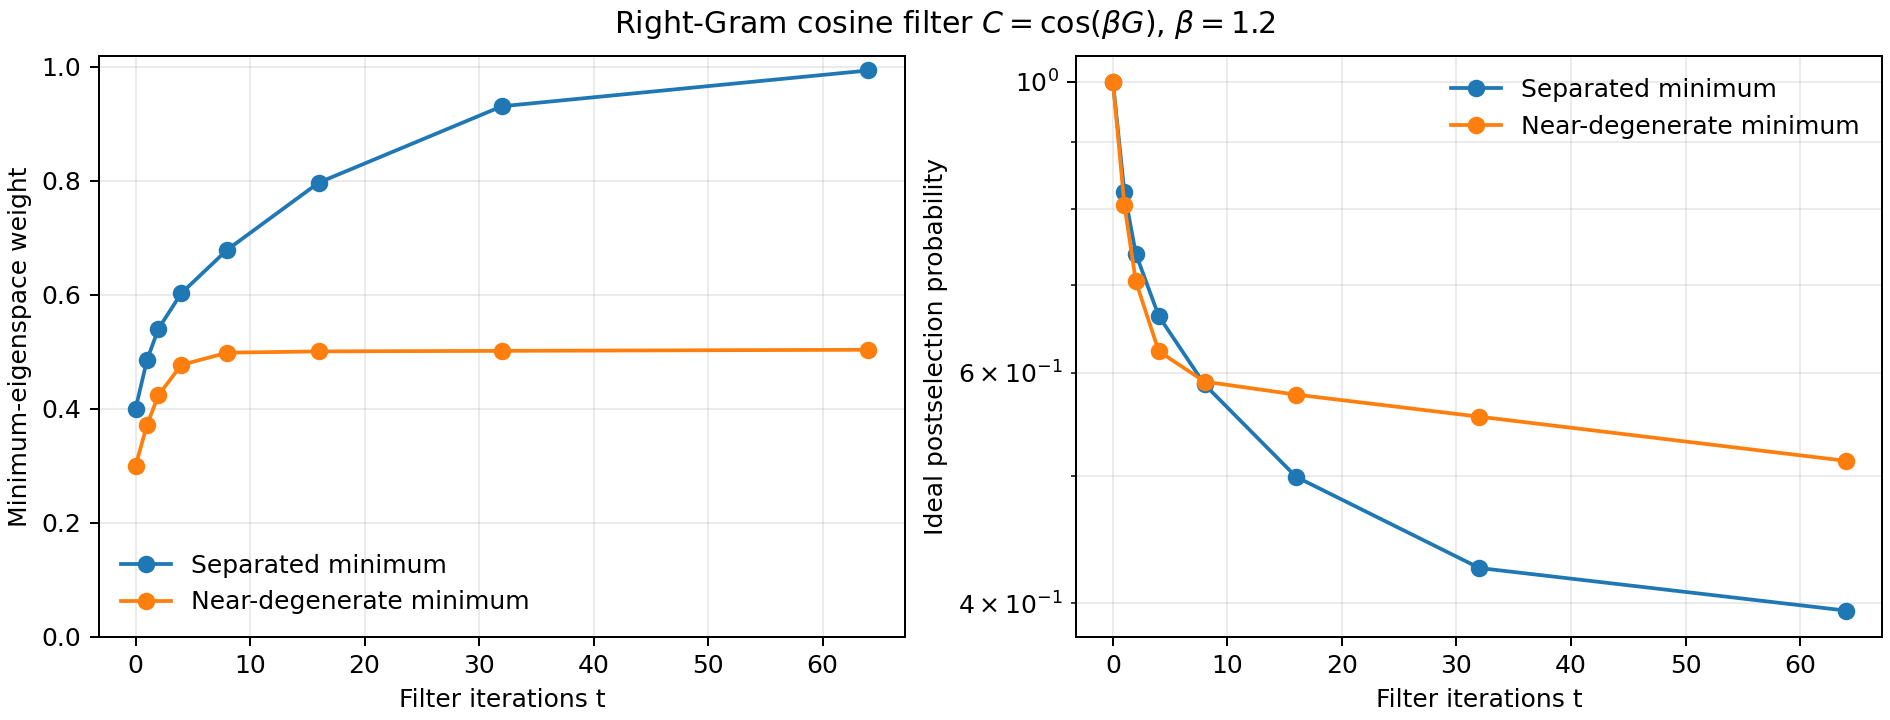
\includegraphics[width=\linewidth]{../../figures/qmsve_matrix_level.png}
\caption{Exact matrix-level conditional target weight and ideal filter success probability. The separated case concentrates on the minimum eigenspace; the near-degenerate case does not do so over the displayed iteration range.}
\label{fig:filter}
\end{figure}

\begin{center}
\scriptsize
\begin{tabular}{lrrrrr}
\toprule
Case & $\sigma_{\min}$ & $a_{\min}$ & $G^8$ estimate & $\cos(\beta G)^8$ estimate / mass & $\cos(\beta\sqrt G)^8$ estimate / mass\\
\midrule
Square, separated & 0.12 & 0.40 & 0.8600 & 0.2896 / 0.6791 & 0.1643 / 0.9417\\
Near-degenerate & 0.20 & 0.30 & 0.8000 & 0.2076 / 0.4987 & 0.2027 / 0.5059\\
Degenerate minimum & 0.20 & 0.40 & 0.7000 & 0.2713 / 0.9254 & 0.2041 / 0.9963\\
Zero target overlap & 0.12 & 0 & 0.8600 & 0.4809 / 0 & 0.4803 / 0\\
Wide, full row rank & 0 & 0.16 & 0.8000 & 0.2744 / 0.5666 & 0.1442 / 0.8715\\
Rank-deficient square & 0 & 0.30 & 0.8000 & 0.2654 / 0.5714 & 0.1435 / 0.8719\\
Rotated tall, full column rank & 0.15 & 0.35 & 0.6500 & 0.3065 / 0.8214 & 0.1630 / 0.9898\\
\bottomrule
\end{tabular}
\end{center}
\noindent The $G^8$ column reports the estimated largest singular value; the cosine columns report the estimated smallest singular value and conditional minimum-eigenspace mass. For the square-gap case, $G^8$ has ideal success probability $0.00200$, whereas the cosine-Gram response has success probability $0.5876$. This distinction prevents a conditional estimate from being mistaken for a low-cost accepted sample.

For the square-gap example, finite-degree Taylor responses at $t=8$ give:
\begin{center}
\small
\begin{tabular}{rrrrrr}
\toprule
Degree in $G$ & Degree in $\sigma/\alpha$ & Uniform error bound & $\widehat\sigma$ & Target mass & Ideal success probability\\
\midrule
2 & 4 & $1.591\times10^{-1}$ & 0.2891 & 0.6801 & 0.1558\\
4 & 8 & $8.260\times10^{-3}$ & 0.2896 & 0.6791 & 0.5499\\
6 & 12 & $2.133\times10^{-4}$ & 0.2896 & 0.6791 & 0.5866\\
12 & 24 & $2.946\times10^{-10}$ & 0.2896 & 0.6791 & 0.5876\\
\bottomrule
\end{tabular}
\end{center}
\noindent These are polynomial-response evaluations with a global analytic boundedness margin. They are not phase-angle synthesis results; the table reports the idealized spectral success probability, not a compiled-circuit success measurement.

At $t=64$, the separated spectrum $(0.12,0.48,0.86)$ has minimum-eigenspace mass $0.994$ and ideal filter success probability $0.395$ under the original cosine-Gram response. The near-degenerate case $(0.20,0.205,0.80)$ reaches only mass $0.504$ with success probability $0.514$. A degenerate minimum with initial subspace mass $0.40$ reaches mass greater than $0.999999$; the method selects the eigenspace, not a unique vector. If the initial state has zero mass on the minimum eigenspace, the filter never creates that component: in the tested instance the estimate remains at $0.48$ while the ideal success probability falls to $0.00282$.

The matrix-level model also shows why a right-space definition matters. A wide full-row-rank matrix has a right-kernel eigenvalue zero in $G$; the method targets that kernel rather than the smallest nonzero singular value. The rank-deficient square example likewise converges toward its zero singular value. A normalization check rejects a matrix whose norm exceeds the declared $\alpha=1$.

For the separated case at $t=8$, the exact filtered Gram mean is $0.08385$. The 2,000-shot Bernoulli estimate is $0.0780$, within the stated 95\% Hoeffding radius $0.03037$. The expected number of fresh filter attempts for these accepted samples is approximately 3,404 under the ideal model. This is a scalar shot-noise check, not a circuit experiment.

The distinct dilation response $\cos(\beta\sigma)$ concentrates faster on the separated example (target mass $0.996$ at $t=16$ versus $0.797$ for $\cos(\beta\sigma^2)$), but its success probability is lower ($0.288$ versus $0.500$). For the near-degenerate example both responses remain close to $0.5$ at $t=16$. These numbers compare exact spectral responses only: their polynomial degrees, encodings, and compiled costs are not matched.


\section{Discussion and limitations}
The finite-spectrum argument isolates the mechanism behind the triangular iteration: a strictly largest filter response on the target eigenspace yields geometric suppression of all other spectral weight. The same calculation applies to other diagonalizable filters under the same response-ratio condition, so the leakage inequality itself should be read as an elementary filter bound, not as a new quantum algorithmic primitive. The practical question is whether a chosen response can be implemented at a useful polynomial degree and whether enough accepted samples can be obtained within the available depth and query budget. This report does not answer that end-to-end optimization problem.

The result has several explicit assumptions. The target component must have nonzero initial mass; a useful guarantee requires a quantitative lower bound on that mass. A strict response ratio $r<1$ is needed, which for the cosine-Gram filter follows from a nonzero spectral gap above the minimum eigenvalue. Repeated postselection incurs expected overhead $1/Z_t$, and the success probability can shrink exponentially with $t$ when the target eigenvalue is positive. The normalization $\alpha$ must be known and its acquisition cost is not included. The polynomial Taylor proxy is bounded on the assumed block-encoding spectrum, but no QSVT phases are generated and no finite-precision or synthesis error is propagated through $t$ iterations. The readout analysis assumes ideal independent Bernoulli trials and a prepared accepted state.

The numerical examples are deliberately small and chosen to expose degeneracy, small gaps, zero overlap, and kernel effects. They do not establish performance on chemistry instances, large sparse matrices, or hardware. In particular, no speedup, improved query complexity, or novelty over existing power methods and polynomial filtering is claimed. A resource comparison would need to fix a common input model and include state preparation, normalization, block-encoding, filter degree, success amplification or restart, readout shots, and finite-precision errors.

\section{Conclusion}
We gave an assumption-explicit formulation of a cosine-based minimum-singular-value iteration on the normalized right Gram operator and stated its conditional finite-spectrum convergence and Bernoulli readout guarantees. We separated the $\cos(\beta\sigma^2/\alpha^2)$ Gram response from a distinct $\cos(\beta\sigma/\alpha)$ response, and audited both on seven small spectral examples. The examples confirm the role of gap, target overlap, degeneracy, and right-kernel support. They also show why conditional convergence alone is insufficient to establish an efficient algorithm: success probability and implementation cost must be counted. Establishing a useful end-to-end resource advantage remains open in this study.

\appendix
\section{Proof of the finite-spectrum bounds}\label{app:proof}
Write $Q_T=\sum_{i\in T}p_iq_*^{2t}$ for the unnormalized target weight and $Q_{\perp}=\sum_{i\notin T}p_iq_i^{2t}$. The assumed response bound implies
\[
 Q_{\perp}\leq r^{2t}q_*^{2t}\sum_{i\notin T}p_i
 = (1-a)r^{2t}q_*^{2t},\qquad
 Q_T=aq_*^{2t}.
\]
Since $F_t=Q_T/(Q_T+Q_{\perp})$, we have
\[
 1-F_t=\frac{Q_{\perp}}{Q_T+Q_{\perp}}
 \leq\frac{Q_{\perp}}{Q_T}
 \leq\frac{1-a}{a}r^{2t}.
\]
Every eigenvalue outside $T$ lies in $[\lambda_0,1]$, so the filtered mean satisfies
\[
 0\leq\mu_t-\lambda_0
 =\sum_{i\notin T}\frac{p_iq_i^{2t}}{Z_t}(\lambda_i-\lambda_0)
 \leq(1-F_t)(1-\lambda_0)
 \leq\frac{1-a}{a}r^{2t}.
\]
For a readout estimate with $|\widehat\mu_t-\mu_t|\leq\zeta$, clipping to $[0,1]$ cannot increase its distance from $\lambda_0\in[0,1]$. Thus $|\widehat\mu_t-\lambda_0|\leq\mu_t-\lambda_0+\zeta$. For nonnegative $x,y$, $|\sqrt{x}-\sqrt{y}|\leq\sqrt{|x-y|}$, giving the stated singular-value error bound after multiplication by $\alpha$.

\section{Lean formalization status}\label{app:lean}
The exact finite-weight postselection inequality and its posterior-moment consequence are checked in Lean 4. The formal source is reproduced in Appendix~\ref{app:lean-source}; it was checked with Lean 4.35.0 and Mathlib v4.35.0 using \texttt{lake build QMSVE} and \texttt{lake env lean Audit.lean}, both with exit code 0. The matrix spectral decomposition, identification of filter weights with matrix eigencomponents, QSVT implementation, and Bernoulli concentration remain outside the scalar formalization.

\section{Source manuscript metadata}
The QMSVE source used for this reassessment is the supplied manuscript titled \emph{Quantum maximum/minimum singular-value estimation algorithms}. The copy examined does not state author, venue, or publication metadata, and labels the triangular iteration as provisional. The manuscript's author field is consequently left as a placeholder in the main file; no identity or affiliation is inferred.

\section{Lean source code}\label{app:lean-source}
The following is the complete formal source used for the two scalar statements above. Its imports are pinned by the adjacent Lean project files.
\VerbatimInput[fontsize=\tiny,breaklines=true]{../../lean/QMSVE.lean}

% Reference tail (merge with the integrated bibliography and retain the keys).
\begin{thebibliography}{9}
\bibitem{QMSVE} \emph{Quantum maximum/minimum singular-value estimation algorithms}. Unpublished manuscript supplied as \texttt{2023\_0311\_QMSVE.pdf}; author and publication metadata unstated in the copy examined.
\bibitem{Gilyen} A. Gily\'en, Y. Su, G. H. Low, and N. Wiebe, ``Quantum singular value transformation and beyond: exponential improvements for quantum matrix arithmetics,'' in \emph{Proceedings of the 51st Annual ACM SIGACT Symposium on Theory of Computing}, pp. 193--204 (2019), doi:10.1145/3313276.3316366; arXiv:1806.01838.
\bibitem{SekiYunoki} K. Seki and S. Yunoki, ``Quantum Power Method by a Superposition of Time-Evolved States,'' \emph{PRX Quantum} \textbf{2}, 010333 (2021), doi:10.1103/PRXQuantum.2.010333; arXiv:2008.03661.
\bibitem{Kyriienko} O. Kyriienko, ``Quantum inverse iteration algorithm for programmable quantum simulators,'' \emph{npj Quantum Information} \textbf{6}, 7 (2020), doi:10.1038/s41534-019-0239-7; arXiv:1901.09988.
\bibitem{Nghiem} N. A. Nghiem, H. Sukeno, S. Zhang, and T.-C. Wei, ``Improved Quantum Power Method and Numerical Integration Using Quantum Singular Value Transformation,'' \emph{Physical Review A} \textbf{111}, 012434 (2025), doi:10.1103/PhysRevA.111.012434; arXiv:2407.11744.
\bibitem{QCG2023} K. Toyoizumi, S. Yamamoto, and Y. Hoshino, ``Hamiltonian simulation using quantum singular value transformation: complexity analysis and application to the linearized Vlasov-Poisson equation,'' arXiv:2304.08937, version 2 (2023).
\bibitem{QCG2024} K. Toyoizumi, K. Wada, S. Yamamoto, and Y. Hoshino, ``Quantum conjugate gradient method using the positive-side quantum eigenvalue transformation,'' arXiv:2404.02713, version 2 (2024).
\end{thebibliography}
\end{document}
